\section{Com funcionen els dispositius electrònics}
Els dispositius electrònics com els telèfons mòbils, tauletes, ordinadors, caixers automàtics, consoles, impressores, rentaplats, televisions, rentadores, microones, robots, ràdios... tots resolen tasques diferents, i tenen utilitats diferents, però tots funcionen fonamentalment de la mateixa manera. 

\subsection{Com interactuem amb els dispositius electrònics}
Els dispositius són màquines que responen a accions com ara tocar la pantalla tàctil, clicar amb el ratolí, escriure amb el teclat, parlar pel micròfon, prémer algun botó del comandament a distància... i, el dispositiu et genera una resposta en funció de l'acció que hagis fet: pot canviar el contingut de la pantalla, reproduir un so a través dels altaveus, enviar un senyal a un altre dispositiu, canviar el canal de la televisió, retirar una quantitat de diners...

La informació que dones al dispositiu l'anomenarem \textbf{entrada}. I al resultat o resposta que et genera l'anomenarem \textbf{sortida}. 

Per exemple, quan premem el botó d'apujar el volum del comandament de la televisió, estàs generant una entrada. La televisió la processa i genera una sortida en funció de l'entrada, és a dir, apuja el volum. Si l'entrada fos diferent i haguéssim premut el botó de canviar de canal, la sortida també seria diferent, i s'hauria canviat el canal en lloc d'apujar el volum. Podem deduir doncs que la sortida depèn completament de l'entrada. Si canviem l'entrada, la sortida també serà diferent.

Els components de l'ordinador en si no poden processar les entrades i generar sortides, es necessita algun element que rebi la informació (entrada), la processi i generi el resultat (sortida). Aquí és on entra la programació. Els programes processen la informació i donen les ordres als components per generar una sortida.

Per exemple, premem el botó d'engegar del mòbil (entrada), l'entrada arriba al programa, aquest processa la informació i genera una sortida, la qual consisteix a encendre la pantalla del mòbil.

\begin{figure}[h]
    \centering
    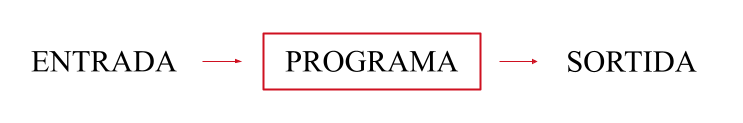
\includegraphics[width=.7\textwidth]{capitols/figures/i_o prog.png}
    \caption[Diagrama d'entrada, programa i sortida.]{Diagrama d'entrada, programa i sortida. Font: elaboració pròpia.}
    \label{Figura}
\end{figure}

Totes les tasques que podem resoldre utilitzant un programa les anomenarem problema. Ens referim a tots els exemples d'aquest punt com a un problema que hem resolt amb un programa. 

Quan parlem d'un problema matemàtic com ara sumar dos nombres, la solució és el resultat de la suma, l'equivalent a la sortida. Però quan parlem de problemes de programació, com els d'aquest treball, la solució és el procediment, el qual és diferent de la sortida, ja que la sortida és el resultat de finalitzar el procediment.

\subsection{Que són els algoritmes i en què es diferencien dels programes}
Un algoritme és un procediment, un seguit de passos finits i ordenats que resolen una tasca o problema concret. Els algoritmes ofereixen formes teòriques de resoldre un problema.

% treure llenguatge de programació
En canvi, un programa és tot allò que un ordinador pot entendre i executar. Un programa pot implementar\footnote{La paraula 'implementar' s'utilitza en aquest context per expressar l'acció de passar alguna solució/procediment/algoritme a un programa. La implementació d'un algoritme és un programa que resolgui la mateixa tasca que l'algoritme implementat.} o \quotes{traduir} un algoritme. Els programes ofereixen formes pràctiques de resoldre un problema.

És a dir, els algoritmes són el procediment o els passos a seguir. I els programes són la traducció dels algoritmes de manera que els ordinadors ho puguin entendre i executar.
%traduir
% Aquests conceptes que he explicat fins ara ens els trobem diàriament. Per exemple, quan volem cuinar un plat de pasta, necessitem diversos elements: ingredients, una recepta i un cuiner. Amb la recepta tenim la teoria de com hem de cuinar per tenir el plat de pasta, el cuiner executa la recepta, i depenent del tipus de pasta que utilitzi obtindrà plats diferents. Si la recepta diu que s'han d'utilitzar macarrons, només podràs fer un plat de macarrons. En canvi, si diu que es pot utilitzar qualsevol classe de pasta, podràs seguir aquesta recepta tant per fer espaguetis com macarrons.

% Amb els ordinadors passa el mateix. Quan volem resoldre un problema com cuinar un plat de pasta, necessitem: entrades, un algoritme i un programa. Amb l'algoritme (recepta) tenim la teoria de com resoldre el problema, el programa seria el cuiner, ja que aplica l'algoritme o teoria i resol el problema a la pràctica. Finalment, les entrades serien els ingredients, i depenent de les entrades obtindrem diferents sortides, igual que amb diferents tipus de pasta podem obtenir diferents plats o sortides. Podem seguir la mateixa recepta amb diferents tipus de pasta i, per tant, el cuiner farà el mateix. Igual que pots utilitzar el mateix algoritme i programa amb diferents entrades i la sortida dependrà de l'entrada. Ja que si cuines amb macarrons, no obtindràs espaguetis.

Per exemple, hi ha el següent problema que volem resoldre amb un programa: agafem tres nombres que anomenem $x, y, z$ i volem trobar $(x+y)\cdot z$. Aquest problema està generalitzat perquè no tenim valors fixos per l'entrada i, per tant, no podem saber quina és la sortida. És a dir, farem un algoritme i programa que funcionin per a qualsevol nombre, no només un.

Per solucionar matemàticament aquest problema, primer cal resoldre la suma, i després la multiplicació. I per fer un programa que el resolgui, podríem fer el següent:

ALGORITME:
\begin{enumerate}
    \item Llegir els nombres amb l'ordre adequat.
    \item Sumar els dos primers nombres.
    \item Multiplicar el resultat del pas 2 pel tercer nombre.
    \item La solució és el resultat del pas 3.
\end{enumerate}

PROGRAMA:
\begin{figure}[h]
    \begin{minted}[
    frame=lines,
    framesep=2mm,
    baselinestretch=1.2,
    bgcolor=LightGray,
    fontsize=\footnotesize,
    linenos
    ]{python}
    x = int(input())    # agafar l'entrada i assignar-li el valor x
    y = int(input())    # agafar l'entrada i assignar-li el valor y
    z = int(input())    # agafar l'entrada i assignar-li el valor z
    
    a  = x + y          # pas 2 de l'algoritme
    b = a * z           # pas 3 de l'algoritme
    print(b)            # escriure la solució
    \end{minted}
    \caption[Programa que resol l'operació.]{Programa que resol l'operació\footnotemark. Font: elaboració pròpia.}
    \label{Figura}
\end{figure}
\footnotetext{El programa està escrit en Python. El propòsit és fer-se una idea de com és un programa, ja que en parlarem durant tot el treball. No cal entendre la sintaxi del llenguatge de programació. Després dels coixinets hi ha un comentari, text que no afecta el funcionament, només és explicatiu.}

Com podem veure clarament, l'algoritme és un seguit de passos i el programa permet executar l'algoritme en un ordinador ja que ho escriu de forma que els ordinadors ho poden executar. 

També veiem com independentment de les entrades que tinguem, el procediment sempre serà el mateix. En un cas generalitzat com aquest, no tenim entrades i sortides concretes, però podem especificar un cas i d'aquesta manera podem comprovar el correcte funcionament del programa. Posaré un cas concret en què $x = 2, y = 3, z = 4$. En aquest cas, les entrades són 2, 3 i 4 i la sortida seria $(2+3)\cdot4 = 20$.


\subsection{Com se solucionen els problemes més complexos}
En els exemples anteriors hem resolt problemes molt senzills, però quan hem d'abordar problemes més complexos, ens trobarem amb altres dificultats. Pot passar que hi hagi moltes solucions diferents que resolen el problema, i hi haurà solucions poc eficients que haurem d'identificar i descartar. És molt important analitzar l'eficiència de les solucions per saber si és profitós executar-les. Si saps que el programa tardarà anys en acabar les operacions, podràs considerar si val la pena fer-lo.

Precisament en aquest treball ens centrarem a trobar diverses solucions per a un problema i analitzar-les per saber la seva complexitat en funció de la quantitat de dades de l'entrada. Ho explicaré més detalladament en el següent apartat. Ara per fer-nos una idea que un problema té diverses solucions unes més eficients que les altres, posaré un exemple.

El problema consisteix a fer un programa que trobi la solució a qualsevol sudoku\footnote{Aquest és un trencaclosques en què l'objectiu és omplir amb números de l'1 al 9 una quadrícula de 9x9 caselles dividida en quadres de 3x3. Les úniques restriccions són que no es poden repetir números en cap filera, columna o quadre 3x3. Inicialment, el trencaclosques et proporciona alguns nombres col·locats a la seva casella corresponent i l'objectiu és trobar-ne la resta.}. Hi ha moltes estratègies que es poden seguir per resoldre'n un, seguidament en proposo dues. 

La primera estratègia és posar tots els nombres a l'atzar i comprovar cada vegada si la solució és vàlida, i repetir el procés fins a trobar la combinació correcta. Quan apliquéssim aquest algoritme en un programa, aquest seria molt lent, perquè hi ha moltes combinacions possibles, i inclús podríem repetir combinacions que ja haguéssim provat.

La segona estratègia és la següent: Posem un nombre, escollit de forma ordenada, en una casella buida. Seguidament, comprovem que la fila, columna, i el quadre ens ho permeti, en el cas que sigui vàlid, repetim el procés amb la següent casella buida, i, si no és vàlid, provem amb un nombre diferent. Amb aquesta solució estem provant nombres de forma ordenada i sense repetir-los. Aquesta solució la podem generalitzar de la següent manera: si funciona avancem un pas i repetim el procés, si no funciona retrocedim i repetim el procés provant el següent nombre. Aquest tipus de solució és un algoritme de \textit{backtracking}. La implementació d'aquesta solució es pot veure a \textcolor{red}{l'annex 1}.

\section{Quina és la millor solució?}
Quan podem solucionar un mateix problema de diverses maneres, el més lògic és resoldre'l de la manera més ràpida i eficient possible. Sinó, totes les tasques tardarien molt més a acabar i el resultat seria un dispositiu molt lent. Per evitar això hem d'analitzar l'eficiència o complexitat dels algoritmes.

\subsection{Introducció a l'anàlisi de l'eficiència dels algoritmes}%----------------------------------------
L'eficiència dels algoritmes o complexitat algorítmica és una mesura per determinar com d'eficient és un algoritme o programa. Amb aquesta mesura podem comparar els algoritmes o programes entre ells i determinar quin és més convenient d'utilitzar. La complexitat algorítmica depèn únicament de dos paràmetres que s'estudien per separat:
\begin{enumerate}
    \item L'\textbf{eficiència temporal} (la velocitat de l'algoritme).
    \item L'\textbf{eficiència espacial} (la quantitat de memòria que ocupa).
\end{enumerate}

L'eficiència espacial fa referència a l'espai que ocupen les dades, les dades d'entrada s'han d'emmagatzemar perquè el programa les pugui utilitzar, i l'algoritme pot requerir emmagatzemar-ne més. Com més dades s'hagin d'emmagatzemar direm que l'algoritme té una pitjor eficiència espacial o major complexitat. Però en aquest treball només ens centrarem en l'eficiència temporal. 

L'eficiència o complexitat temporal mesura quant tardarà en acabar una tasca un algoritme o programa en funció de la mida de l'entrada. 

Per exemple: hi ha un dentista que tarda 30 minuts per visitar un pacient. Per tant, per saber quan acabarà la feina només hem de multiplicar el nombre de pacients per 30 minuts. Si anomenem $n$ el nombre de pacients, podem saber que el dentista treballarà $30 \cdot n$ minuts. D'aquesta manera estem expressant en funció del nombre de pacients ($n$) el temps que treballarà el dentista. 

La complexitat algorítmica temporal mesura el mateix. En funció de la quantitat de dades de l'entrada ($n$), expressa quant tardarà l'algoritme o programa en acabar.

L'eficiència temporal es pot analitzar de dues formes:
\begin{enumerate}
    \item De forma \textbf{matemàtica}. Consisteix a analitzar la quantitat d'operacions que fa l'algoritme.
    \item De forma \textbf{empírica}. Implementar l'algoritme i mesurar el temps que tarda el programa. A partir d'aquestes mesures s'intenta predir el comportament del programa, i, per tant, de l'algoritme, per les mesures no realitzades.
\end{enumerate}

Ha de quedar clar que l'eficiència temporal d'un algoritme no depèn en absolut de l'ordinador que utilitzem, sinó en l'algoritme en si mateix, és a dir, en la quantitat d'operacions o comparacions que faci. Un ordinador més potent podrà fer les operacions més ràpidament, però els dos faran la mateixa quantitat d'operacions, és a dir, serà més ràpid, però no més eficient.

Tornant a l'exemple del dentista, si un dentista B tarda 5 minuts per pacient en lloc del dentista A que en tarda 30. El dentista B tardaria $5 \cdot n$ minuts a atendre $n$ pacients. El dentista B aten més ràpidament els pacients, però els dos realitzen el mateix procediment. Per tant, el dentista B és més ràpid, però tots dos són igual d'eficients. 

Per això l'anàlisi matemàtic és més fiable que l'empíric. Perquè el matemàtic depèn únicament de l'estudi de l'algoritme, i en l'empíric hi ha altres factors que afecten el resultat.

% Com que l'eficiència temporal es pot mesurar de dues maneres i arribem al mateix resultat de les dues formes. Per simplicitat i perquè un programa és l'implementació de l'algoritme, a partir d'ara quan em refereixi a analitzar l'eficiència o complexitat d'un algoritme, se sobreenten que pot ser tant l'algoritme com el programa depenent de com s'analitzi.
\begin{figure}[h]
    \centering
    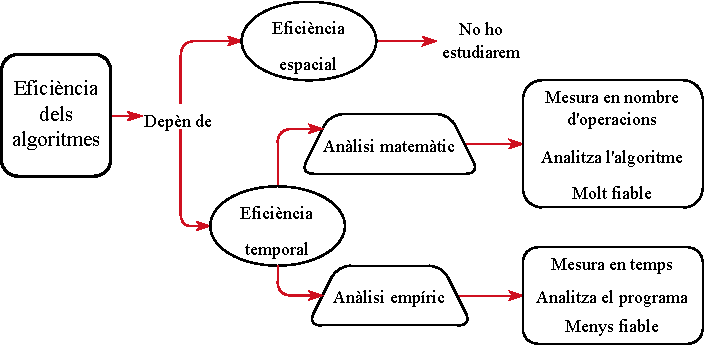
\includegraphics[width=.65\textwidth]{capitols/figures/diagram.drawio (1).pdf}
    \caption[Diagrama de l'eficiència dels algoritmes.]{Diagrama de l'eficiència dels algoritmes. Font: elaboració pròpia.}
    \label{Figura}
\end{figure}


\subsection{Notació de Landau}
Hi ha diverses maneres de mesurar la complexitat algorítmica respecte de l'entrada. Nosaltres utilitzarem la notació de Landau, coneguda també com a O gran o notació asimptòtica.

La notació de Landau proporciona una forma \quotes{aproximada} d'expressar la complexitat d'un algoritme en funció d'$n$ quan $n$ pren valors molt grans. Ens interessa analitzar el pitjor cas possible de l'algoritme perquè ens assegura que independentment del cas, l'algoritme tardarà igual o menys que la complexitat analitzada.

Formalment, la notació de Landau s'utilitza per descriure el comportament asimptòtic de les funcions. Per exemple, si el temps o quantitat de passos necessari per resoldre un problema de mida $n$ ve donat per $f(n) = 3n^2 + 2n -1$. Si eliminem les constants, ja que depenen de l'ordinador on s'executi i, per tant, varien la velocitat però no l'eficiència, i eliminem també els termes de creixement més lent (ja que estem analitzant el $\lim_{n \to \infty} f(n)$). La quantitat d'operacions quedaria determinada per l'expressió $f(n) = n^2$. Per això, vulgarment diem que és un anàlisi aproximat.

En aquesta notació les constants s'eliminen per dos motius: perquè estem analitzant quan $n$ pren valors molt grans, i, per tant, les podem negligir igual que els termes de creixement més lent. I perquè a l'hora d'executar l'algoritme depenent de l'ordinador, compilador, llenguatge de programació, implementació, etc, les constants varien. Per exemple, si la quantitat d'operacions que fa un algoritme ve donada per l'expressió $f(n) = n^2$ i un ordinador A fa 1 operació per segon i un ordinador B fa 4 operacions per segon (un ordinador normal pot fer unes $10^8$ operacions per segon). L'ordinador A tardaria $n^2$ segons, i l'ordinador B tardaria $\frac{n^2}{4}$ segons. Veiem com canviant la velocitat de l'ordinador, però executant el mateix programa i algoritme, obtenim una diferència de velocitat constant. Com que estem analitzant l'eficiència, no la velocitat, podem eliminar les constants.

% En l'exemple anterior del dentista podem veure com les constants (el temps que tarden a atendre cada pacient) poden variar i la quantitat de passos ($n$) que fan els dentistes són els mateixos. Per això, diem que les constants depenen de l'ordinador, i, per tant, es poden eliminar de l'anàlisi d'eficiència.

% No explicaré totes les funcions que es poden expressar en aquesta notació, sinó les més bàsiques i necessàries per a aquest treball. 

\subsubsection*{Complexitat constant $O(1)$}
La primera complexitat és la complexitat constant, i s'expressa de la següent manera: $O(1)$. 

La lletra \quotes{o} majúscula indica la notació que estem utilitzant, per això la notació de Landau també es diu notació O gran. I el que hi ha a l'interior del parèntesi indica el creixement de l'algoritme. En aquest cas hi ha un 1 i no hi ha cap $n$, això vol dir que les operacions no depenen de la mida de l'entrada i sempre, independentment de la seva mida l'algoritme farà la mateixa quantitat d'operacions.

Per exemple, si vols agafar un llibre d'una estanteria d'$n$ llibres i saps que vols el primer. No caldrà que el busquis, podràs agafar el primer fent una única operació. No importa quants llibres hi hagi, sempre faràs una sola operació. Per això, el nombre d'operacions és constant i no depèn d'$n$ (la mida de l'entrada).

Si ara féssim un gràfic d'aquesta complexitat i poséssim a l'eix d'abscisses la mida de l'entrada ($n$), i a l'eix d'ordenades el nombre d'operacions. Obtindríem la figura 1.4.

% -------------------------------------------------------------gràfic complexitat constant
% \begin{wrapfigure}[7]{R}{0.35\textwidth}
\begin{figure}[h]
    % \vspace{-18pt}
    \centering
    \begin{tikzpicture}
        \centering
        \begin{axis}[xmin=0, xmax=100, ymin=0, ymax=8, axis lines = middle, 
        x label style={at={(axis description cs:0.5,-0.1)},anchor=north},
        y label style={at={(axis description cs:-0.1,.5)},rotate=90,anchor=south},
        xlabel={$n$ mida de l'entrada},
        ylabel={nombre d'operacions},
        style={thick}, 
        compat=1.18, width=.35\textwidth]
        \addplot[color=vermellpral, domain=0:100]{1};
        % \addplot[color=verd, domain=0:10]{3};
        \legend{$O(1)$,$O(3)$}
        \end{axis}
    \end{tikzpicture}
    \caption[Gràfic de complexitat constant.]{Gràfic de complexitat constant. Font: elaboració pròpia.}\label{fig:my_label}
\end{figure}

Podem veure com a mesura que l'entrada es va fent cada vegada més gran, el nombre d'operacions es manté constant.

Amb l'anàlisi de complexitats estudiem quant tardarà l'algoritme quan la mida de l'entrada $n$ sigui molt gran. En aquest cas veiem que no creix i que es manté constant. 

Per tant, si hem d'utilitzar un algoritme de complexitat constant per a $n = 1.000.000$, farà la mateixa quantitat d'operacions que per a $n = 10$. I la velocitat d'aquestes operacions dependran completament de factors externs a l'algoritme (ordinador, implementació, etc.).

\subsubsection*{Complexitat lineal $O(n)$}
Aquesta ja depèn de la mida de l'entrada i s'expressa així: $O(n)$. A mesura que incrementa $n$ el temps també incrementa de forma directament proporcional.

Per exemple, si estàs buscant un llibre en una estanteria, hauràs de comprovar cada llibre fins a trobar el que busques. En el pitjor cas possible el llibre estarà situat l'últim a l'estanteria, i hauràs de comprovar-los tots fins a trobar-lo. Si hi ha $n$ llibres, trobar el teu llibre t'haurà costat $n$ operacions com a màxim. Per tant, l'eficiència temporal d'aquest procediment són $n$ operacions, complexitat lineal o $O(n)$.

L'exemple del dentista també té complexitat lineal, ja que fa $n$ visites. Ens és igual si tarden $30 \cdot n$ minuts, $5 \cdot n$ minuts, o qualsevol constant per $n$, ja que creixen de la mateixa manera, linealment. I, perquè en aquesta notació les constants s'eliminen.

En el gràfic 1.5 podem veure que a mesura que incrementa la mida de l'entrada, també incrementa el nombre d'operacions en la mateixa mesura. Per a una mida d'entrada petita el nombre d'operacions incrementa igual de ràpid que per a mides d'entrada més grans. 
% -------------------------------------------------------------gràfic complexitat lineal
% \begin{wrapfigure}[8]{r}{.35\textwidth}
\begin{figure}[H]
% \vspace{-18pt}
\centering
\begin{tikzpicture}
\centering
\begin{axis}[xmin=0, xmax=100, ymin=0, ymax=100, axis lines = middle, 
x label style={at={(axis description cs:0.5,-0.1)},anchor=north},
y label style={at={(axis description cs:-0.1,.5)},rotate=90,anchor=south},
xlabel={$n$ mida de l'entrada},
ylabel={nombre d'operacions},
style={thick}, 
compat=1.18, width=.35\textwidth, 
% legend style={nodes={scale=0.75, transform shape}}, 
legend pos= south east]
\addplot[color=vermellpral, domain=0:100]{x};
\addplot[color=verd, domain=0:100]{5*x};
% \addplot[color=verd, domain=0:10]{3*x};
\legend{$O(n)$, $O(5n)$}
\end{axis}
\end{tikzpicture}
    \caption[Gràfic de complexitat lineal.]{Gràfic de complexitat lineal. Font: elaboració pròpia.}
    \label{fig:my_label}
\end{figure}

% Per tant, un algoritme de complexitat lineal fa tantes operacions com la mida de l'entrada. És a dir, si $n = 10$ farà 10 operacions i si $n = 1.000.000$ farà 1.000.000 d'operacions.

\subsubsection*{Complexitat quadràtica $O(n^2)$}
En aquest tipus d'algoritmes el nombre d'operacions és proporcional al quadrat d'$n$. 

Per exemple, estem al supermercat i tenim una llista de la compra amb $n$ productes. Però abans d'anar a pagar volem comprovar que no ens hàgim deixat res. Així que llegim el primer producte de la llista i el busquem a la nostra cistella, després fem el mateix fins a comprovar els $n$ productes. Cada vegada que busquem el producte a la cistella, estem fent màxim $n$ operacions, és a dir, buscar el producte a la cistella té una complexitat d'$O(n)$. Però estem fent aquest procés tantes vegades com productes apuntats a la llista ($n$). Així que estem fent $n$ operacions $n$ vegades o $n \cdot n = n^2$ operacions. Per tant, l'eficiència temporal d'aquest procediment seria $n^2$ operacions com a màxim.

En el gràfic de la figura 1.6 podem veure clarament com aquesta complexitat és menys eficient que les altres, ja que el nombre d'operacions incrementa molt ràpidament. A diferència de la complexitat anterior, aquesta quan la mida de l'entrada és més petita incrementa més lentament, però a mesura que l'entrada és més gran, el nombre d'operacions incrementa cada vegada més ràpidament. 
% ------------------------------gràfic complexitat lineal
% \begin{wrapfigure}[8]{r}{.35\textwidth}
\begin{figure}[h]
    \centering
    % \vspace{-18pt}
\begin{tikzpicture}
\centering
\begin{axis}[xmin=0, xmax=100, ymin=0, ymax=100, axis lines = middle, 
x label style={at={(axis description cs:0.5,-0.1)},anchor=north},
y label style={at={(axis description cs:-0.1,.5)},rotate=90,anchor=south},
xlabel={$n$ mida de l'entrada},
ylabel={nombre d'operacions},
style={thick}, 
compat=1.18, width=.35\textwidth, 
% legend style={nodes={scale=0.75, transform shape}}, 
legend pos=south east]
\addplot[color=vermellpral, domain=0:10, samples=150]{x^2};
% \addplot[color=verd, domain=0:10]{2*(x^2)};
\legend{$O(n^2)$, $O(2 \cdot n^2)$}
\end{axis}
\end{tikzpicture}
    \caption[Gràfic de complexitat quadràtica.]{Gràfic de complexitat quadràtica. Font: elaboració pròpia.}
    \label{fig:my_label}
\end{figure}

% Per aquesta complexitat podem predir que per a $n = 10$, farà $n^2 = 10^2 = 100$ operacions i per a $n = 1.000.000$ farà $n^2 = 1.000.000^2 = 10^{12}$ operacions. 

Recordem que sempre estem analitzant el pitjor cas possible, així que un algoritme mai farà més operacions de les previstes, però molts cops en farà menys.

\subsubsection*{Complexitat logarítmica $O(\log_2{n})$}
Un algoritme té complexitat logarítmica quan la quantitat d'operacions és proporcional al logaritme d'$n$.

Per exemple: quan busquem una paraula en un diccionari a paper. Per buscar-la primer obrim el diccionari més o menys per la meitat i per ordre alfabètic deduïm si la paraula queda a la dreta o a l'esquerra. Després fem exactament el mateix, però amb una de les meitats i a poc a poc anem fent més petit el rang on podem trobar la paraula. Aquest procés té complexitat logarítmica o $O(\log_2{n})$.

Els logaritmes són la inversa de l'exponencial (una constant elevada a $n$, com $2^n$), i responen a quantes vegades ($v$) la base ($b$) es multiplica a ella mateixa fins a arribar a l'argument ($n$). És a dir $\log_b{n} = v \iff b^v = n$, per exemple: $\log_2{16} = 4 \iff 2^4 = 16$. 

En l'exemple del diccionari per a $n = 16$ partim les pàgines per la meitat, després fem la meitat de la meitat... Així: $16 \rightarrow 8 \rightarrow 4 \rightarrow 2 \rightarrow 1$. Si ens hi fixem, aquesta seqüència és la mateixa que $2^4$ però invertida: $2^4 = 2 \cdot 2^3 = 4 \cdot 2^2 = 8 \cdot 2 = 16$. 

El procediment del diccionari parteix les pàgines exponencialment però de forma inversa, i el logaritme és la inversa de l'exponencial. Per això aquest procediment té complexitat logarítmica.

Una altra forma de resoldre un logaritme és dividir l'argument entre la base $v$ vegades fins a obtenir el quocient d'1. $v$ és el resultat del logaritme. En la figura 1.7 podem veure un exemple amb $\log_2{8} = 3$. És a dir, es necessiten 3 passos per partir 8 dades en 2 meitats fins a obtenir grups d'una dada.
%\begin{wrapfigure}[6]{L}{.4\textwidth}
\begin{figure}[H]
    % \vspace{-18pt}
    \centering
    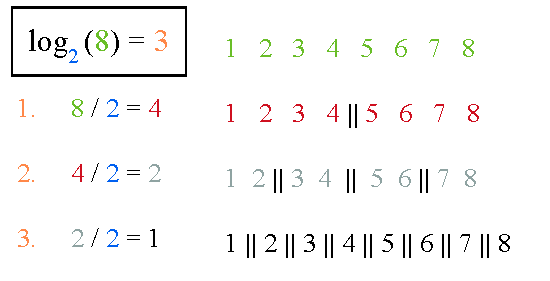
\includegraphics[width=.4\textwidth]{capitols/figures/log (4).pdf}
    % \vspace{-25pt}
    \caption[Relació entre partir nombres i els logaritmes.]{Relació entre partir nombres i els logaritmes. Font: elaboració pròpia.}
    \label{fig:my_label}
\end{figure}
Si el diccionari té $n$ pàgines i $n = 128$, seguint el procediment de l'exemple anterior, haurem de fer $\log_2{n} = \log_2{128} = 7$ passos per arribar a partir-ho en pàgines individuals.  Per això diem que la complexitat d'aquest algoritme és $O(\log_2{n})$.

Si representem aquesta complexitat en el gràfic 1.8, podem veure que quan la mida de l'entrada és més petita, el nombre d'operacions creix més ràpidament, però a mesura que les $n$ són més grans, cada vegada el nombre d'operacions creix més a poc a poc.
% ------------------------------gràfic complexitat log
% \begin{wrapfigure}[8]{R}{.35\textwidth}
\begin{figure}[h]
    \centering
    % \vspace{-18pt}
\begin{tikzpicture}
\centering
\begin{axis}[xmin=0, xmax=100, ymin=0, ymax=100, axis lines = middle, 
x label style={at={(axis description cs:0.5,-0.1)},anchor=north},
y label style={at={(axis description cs:-0.1,.5)},rotate=90,anchor=south},
xlabel={$n$ mida de l'entrada},
ylabel={nombre d'operacions},
style={thick}, 
compat=1.18, width=.35\textwidth]
\addplot[color=vermellpral, domain=-2:100, samples=100]{log2(x)};
\legend{$O(\log_2{n})$}
\end{axis}
\end{tikzpicture}
    \caption[Complexitat logarítmica.]{Complexitat logarítmica. Font: elaboració pròpia.}
    \label{fig:my_label}
\end{figure}



Per tant, per a $n = 10$, farà $\log_2{n} = \lceil\log_2{10}\rceil = 4$ operacions i per a $n = 10^6$ farà $\log_2{n} = \lceil\log_2{10^6}\rceil = 20$ operacions.

\subsubsection*{Totes les complexitats}
Finalment, per comparar les diferents complexitats entre elles, podem fer un gràfic que les representi a totes i una taula amb algunes dades per comparar-les. D'aquesta manera podem veure clarament com la complexitat quadràtica és la pitjor de les que hem explicat, i la complexitat logarítmica és la millor excloent-hi la constant.

Els algoritmes de complexitat constant només es poden utilitzar per a problemes que no depenguin d'$n$, els quals són molt poc comuns i molt senzills, com per exemple operacions matemàtiques. L'algoritme de la figura 1.2, té complexitat constant.
% \begin{wrapfigure}[11]{R}{.45\textwidth}
%     \vspace{-20pt}
%     \centering
% \begin{tikzpicture}
% \begin{axis}[xmin=0, xmax=100, ymin=0, ymax=100, axis lines = middle, 
% x label style={at={(axis description cs:0.5,-0.1)},anchor=north},
% y label style={at={(axis description cs:-0.1,.5)},rotate=90,anchor=south},
% xlabel={$n$ mida de l'entrada},
% ylabel={nombre d'operacions},
% legend pos=south east, 
% style={thick}, 
% compat=1.18, width=.45\textwidth]
% \addplot[color=vermellpral, domain=0:100]{1};
% \addplot[color=taronja, domain=-2:100]{log2(x)};
% \addplot[color=verd, domain=0:100]{x};
% \addplot[color=blau, domain=0:100]{x^2};
% \legend{$O(1)$,$O(log_{2}n)$, $O(n)$, $O(n^2)$}
% \end{axis}
% \end{tikzpicture}
%     \caption{Gràfic amb totes les complexitats. Font: elaboració pròpia.}
%     \label{fig:my_label}
% \end{wrapfigure}

% En aquest gràfic podem veure com la complexitat quadràtica creix molt ràpidament comparat amb les altres, així que els algoritmes amb aquesta complexitat s'haurien d'evitar, sobretot per a $n$ molt grans. Les complexitats constant i logarítmiques són les més ràpides i seria convenient utilitzar algoritmes amb aquestes complexitats per a $n$ molt grans, ja que el nombre d'operacions creix molt a poc a poc en aquest cas. Si per a resoldre un problema podem escollir entre una solució de complexitat quadràtica o logarítmica, doncs ara ja sabem quina solució escollir; la logarítmica.

% \begin{figure}[H]
%     % \vspace{-20pt}
% \centering
% \begin{minipage}{.5\textwidth}
% \begin{tikzpicture}
% \begin{axis}[xmin=0, xmax=100, ymin=0, ymax=100, axis lines = middle, 
% x label styleS={at={(axis description cs:0.5,-0.1)},anchor=north},
% y label style={at={(axis description cs:-0.1,.5)},rotate=90,anchor=south},
% xlabel={$n$ mida de l'entrada},
% ylabel={nombre d'operacions},
% legend pos=north east,
% style={thick}, 
% legend style={nodes={scale=0.75, transform shape}}, 
% compat=1.18, width=.9\textwidth]
% \addplot[color=vermellpral, domain=0:100, samples=100]{1};
% \addplot[color=taronja, domain=-2:100, samples=100]{log2(x)};
% \addplot[color=verd, domain=0:100, samples=100]{x};
% \addplot[color=blau, domain=0:100, samples=100]{x^2};
% \legend{$O(1)$,$O(log_{2}n)$, $O(n)$, $O(n^2)$}
% \end{axis}
% \end{tikzpicture}
%     \caption[Gràfic amb totes les complexitats.]{Gràfic amb totes les complexitats. \\ Font: elaboració pròpia.}
%     \label{fig:my_label}
% \end{minipage}%
% \begin{minipage}{.5\textwidth}
%     \begin{center}
%     \renewcommand{\arraystretch}{1}
%     \begin{tabular}{| l | * {3}{c|}}\hline
%     %  \diagbox[width=.3\textwidth]{\vspace{10pt}\rotatebox{320}{complex}}{$n$}
%     \diagbox[width=.4\textwidth]{complexitat}{$n$}
%      & 10 & 50.000 & $10^{6}$ \\ 
%      \hline
%      \textit{$O(1)$} & 1 & 1 & 1 \\ 
%      \hline
%      \textit{$O(\log_2{n})$} & 4 & 16 & 20 \\
%      \hline
%      \textit{$O(n)$} & 10 & 50.000 & $10^{6}$ \\ 
%     \hline
%     \textit{$O(n^2)$} & 100 & $25 \cdot 10^8$ & $10^{12}$ \\ 
%     \hline
%     \end{tabular}
%     \end{center}
%     \caption[Taula amb exemples del nombre d'operacions per complexitat.]{Taula amb exemples del nombre d'operacions per complexitat. Font: elaboració pròpia.}
%     \label{fig:my_label}
% \end{minipage}
% \end{figure}

\begin{figure}[H]
    \centering
    \begin{tikzpicture}
    \begin{axis}[xmin=0, xmax=200, ymin=0, ymax=200, axis lines = middle, 
    % x label styleS={at={(axis description cs:0.5,-0.1)},anchor=north},
    y label style={at={(axis description cs:-0.1,.5)},rotate=90,anchor=south},
    xlabel={$n$ mida de l'entrada},
    ylabel={nombre d'operacions},
    legend pos= outer north east,
    style={thick}, 
    % legend style={nodes={scale=0.75, transform shape}}, 
    compat=1.18, width=.45\textwidth]
    \addplot[color=vermellpral, domain=0:200, samples=100]{1};
    \addplot[color=taronja, domain=-2:200, samples=200]{log2(x)};
    \addplot[color=verd, domain=0:200, samples=100]{x};
    \addplot[color=blau, domain=0:40, samples=200]{x^2};
\legend{$O(1)$,$O(log_{2}n)$, $O(n)$, $O(n^2)$}
    \end{axis}
    \end{tikzpicture}
    \caption[Gràfic amb totes les complexitats.]{Gràfic amb totes les complexitats. Font: elaboració pròpia.}
    \label{fig:my_label}
\end{figure}
\begin{figure}[H]
    \centering
    \begin{center}
    \renewcommand{\arraystretch}{.8}
    \begin{tabular}{| l | * {5}{c|}}\hline
    %  \diagbox[width=.3\textwidth]{\vspace{10pt}\rotatebox{320}{complex}}{$n$}
    \diagbox[width=.5\textwidth]{Complexitats}{$n$}
     & 10 & 1.000 & 10.000 & 50.000 & $10^{6}$ \\ 
     \hline
     \textit{$O(1)$} & 1 & 1 & 1 & 1 & 1 \\ 
     \hline
     \textit{$O(\log_2{n})$} & 4 & 10 & 14 & 16 & 20 \\
     \hline
     \textit{$O(n)$} & 10 & 1.000 & 10.000 & 50.000 & $10^{6}$ \\ 
    \hline
    \textit{$O(n^2)$} & 100 & $10^6$ & $10^8$ & $25 \cdot 10^8$ & $10^{12}$ \\ 
    \hline
    \end{tabular}
    \end{center}
    \caption[Taula amb exemples del nombre d'operacions per complexitat.]{Taula amb exemples del nombre d'operacions per complexitat. Font: elaboració pròpia.}
    \label{fig:my_label}
\end{figure}%
\vspace{-18pt}
Aquestes quatre complexitats no són totes, també hi ha la complexitat exponencial ($O(2^n)$) i factorial ($O(n!)$) que són molt pitjors que la quadràtica. No les expliquem per què no calen per als objectius d'aquest treball. També hi ha complexitats que es componen de les complexitats bàsiques que hem explicat. Per exemple, si hi ha un algoritme que fa $n$ vegades un procediment logarítmic, la complexitat serà $O(n \cdot \log_2{n})$. 